\documentclass[11pt]{article}

\usepackage{amsmath}
\usepackage{amssymb}
\usepackage{array}
\usepackage{geometry}
\usepackage{enumitem}
\usepackage{float}
\usepackage{cancel}
\usepackage{graphicx}
\usepackage[labelformat=empty]{caption}
\usepackage[T1]{fontenc}

\geometry{
	a4paper,
 	left=20mm,
 	top=20mm,
}

\setlength{\parindent}{0pt}

\begin{document}

\section{Concurrency}

\subsection{Problems}

\begin{description}[noitemsep]
	\item[bad interleaving] multiple methods executed at the same time which causes results not possible if only one thread were running (due to inconsistent state within the methods)
	\item[data races] weird behaviour usually caused by compiler optimizations (out of order execution, memory reordering) and threads that don't see the same value (due to CPU caches)
\end{description}

\subsection{Blocked Threads}

\begin{description}[noitemsep]
	\item[deadlock] processes are blocked as all of them are waiting for another to proceed
	\item[livelock] competing processes detect a potential deadlock but make no progress while trying to resolve it (constantly changing)
	\item[starvation] process is perpetually denied necessary resources
	\item[convoying] thread holding a resource R is descheduled while other threads queue up waiting for R
	\item[priority inversion] lower priority thread holds a resource R that a high priority thread is waiting on
\end{description}

memory model describes the interactions of threads through memory and their shared use of the data.

\subsection{Solutions}

\begin{description}[noitemsep]
	\item[thread-local] resource only accessible by one thread
	\item[immutable] only read access allowed
	\item[synchronization] mutual exclusion for safe write operations
\end{description}

\subsection{Registers}

\begin{description}[noitemsep]
	\item[register] basic memory object, shared or not, read and write operations
	\item[SWMR] (single writer multiple reader), only one concurrent writer but multiple concurrent readers allowed
	\item[safe register] any read not concurrent with a write returns the current operation, any read concurrent with a write can return any value of the domain of the register
\end{description}

\emph{Hint:} the volatile keyword does not only prevent threads from saving that instance in the cache but also prevent out-of-order execution.

\subsection{Hardware Support}

Most hardware provides atomic registers via the instructions Test and Set/Compare and Swap:
\begin{center}
	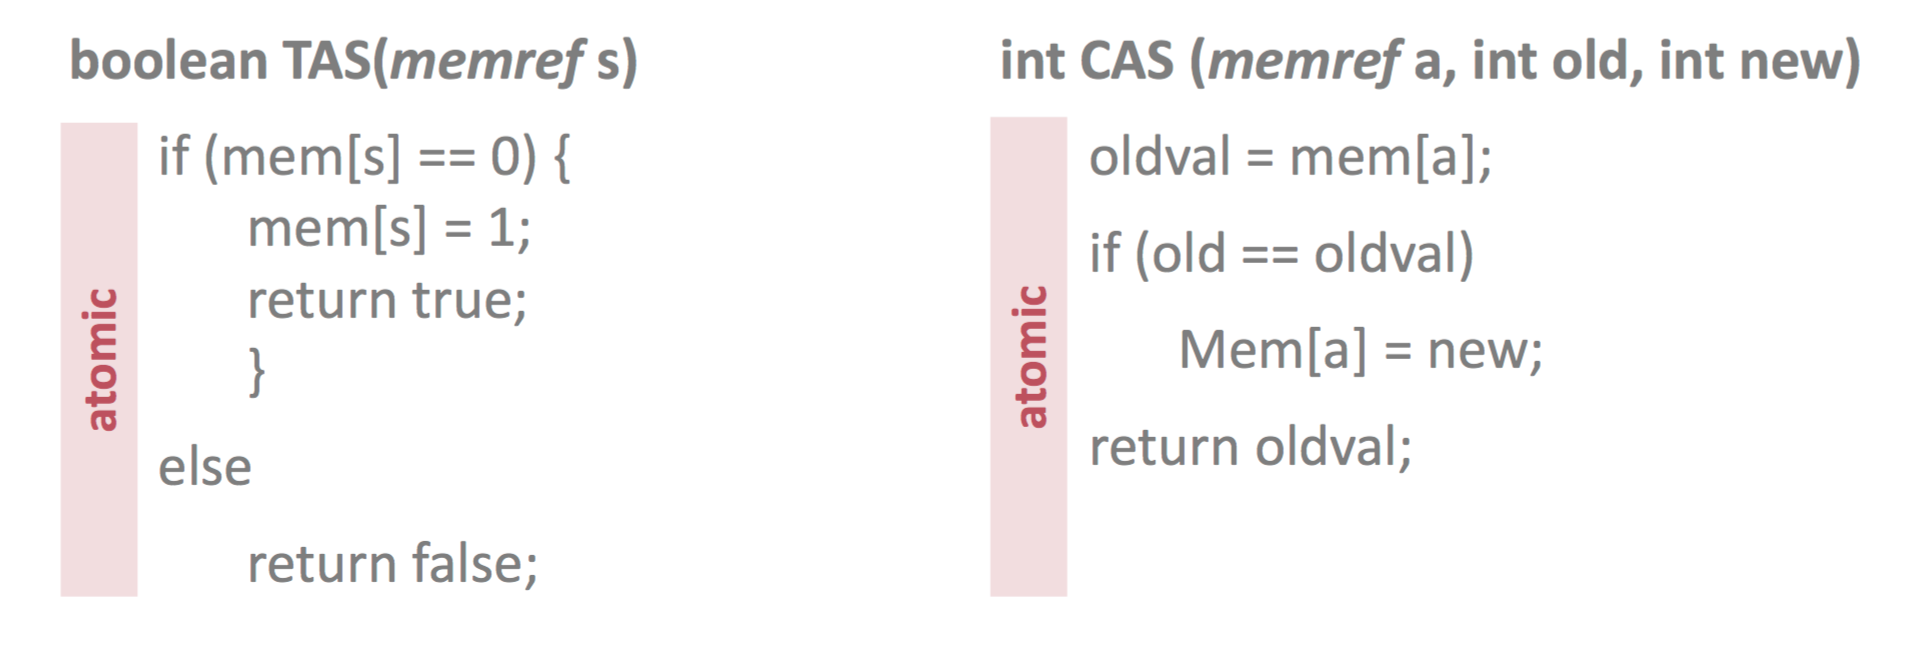
\includegraphics[width=400pt]{images/hardware_support}
\end{center}

\subsection{Deadlock avoidance}

\begin{description}[noitemsep]
	\item[2 phase locking] check if holding a lock would introduce a deadlock, retry if so
	\item[resource ordering] make sure the locks are never held in a way that would cause a deadlock
\end{description}

\subsection{Dining philosphers}

Five silent philosophers sit at a round table with bowls of spaghetti. Forks are placed between each pair of adjacent philosophers.

Each philosopher must alternately think and eat. However, a philosopher can only eat spaghetti when he has both left and right forks. Each fork can be held by only one philosopher and so a philosopher can use the fork only if it is not being used by another philosopher. After he finishes eating, he needs to put down both forks so they become available to others. A philosopher can take the fork on his right or the one on his left as they become available, but cannot start eating before getting both of them.

\subsection{Lock Granularity}

\subsubsection{Coarse Grained}

\begin{description}[noitemsep]
	\item[procedure] lock whole data structure
	\item[advantages] easy to implement
	\item[disadvantages] bottleneck, locks whole data structure
\end{description}

\subsubsection{Fine Grained}

\begin{description}[noitemsep]
	\item[procedure] hand-over-hand traversal
	\item[disadvantages] lots of (un)locking
\end{description}

\subsubsection{Optimistic List}

\begin{description}[noitemsep]
	\item[procedure] 1. find element 2. lock it and predecessor 3. verify
	\item[advantages] no contention on traversals, traversals are wait free, less lock acquisitions
	\item[disadvantages] need to traverse list twice, contains() needs to acquire locks
\end{description}

\subsubsection{Lazy List}

\begin{description}[noitemsep]
	\item[procedure] remove nodes lazily (marking it first)
	\item[advantages] traverses only once, contains() never blocks
\end{description}

\subsubsection{Lockfree List}

\begin{description}[noitemsep]
	\item[procedure] use DCAS (double CAS) to implement lazy list in a lock free manner (allows us to atomically check two conditions at once)
\end{description}

\subsubsection{Lockfree Programming}

\begin{description}[noitemsep]
	\item[lock-freedom] at least one algorithm always makes progress even if other algorithms run concurrently. Implies systemwide progress but not freedom from starvation. Deadlock-free by design.
	\item[wait-freedom] all algorithms return in a finite time. Implies freedom from starvation and lock-freedom.
	\item[non-blocking] failure or suspension of one thread cannot cause failure or suspension of another thread
\end{description}

\paragraph{ABA-Problem}

The ABA problem occurs when one activity fails to recognise that a single memory location was modified temporarily by another activity and therefore erroneously assumes that the overall state has not been changed. \\

Can be solved using DCAS (not available on most platforms), pointer tagging (only delays it) or hazard pointers.

\begin{center}
	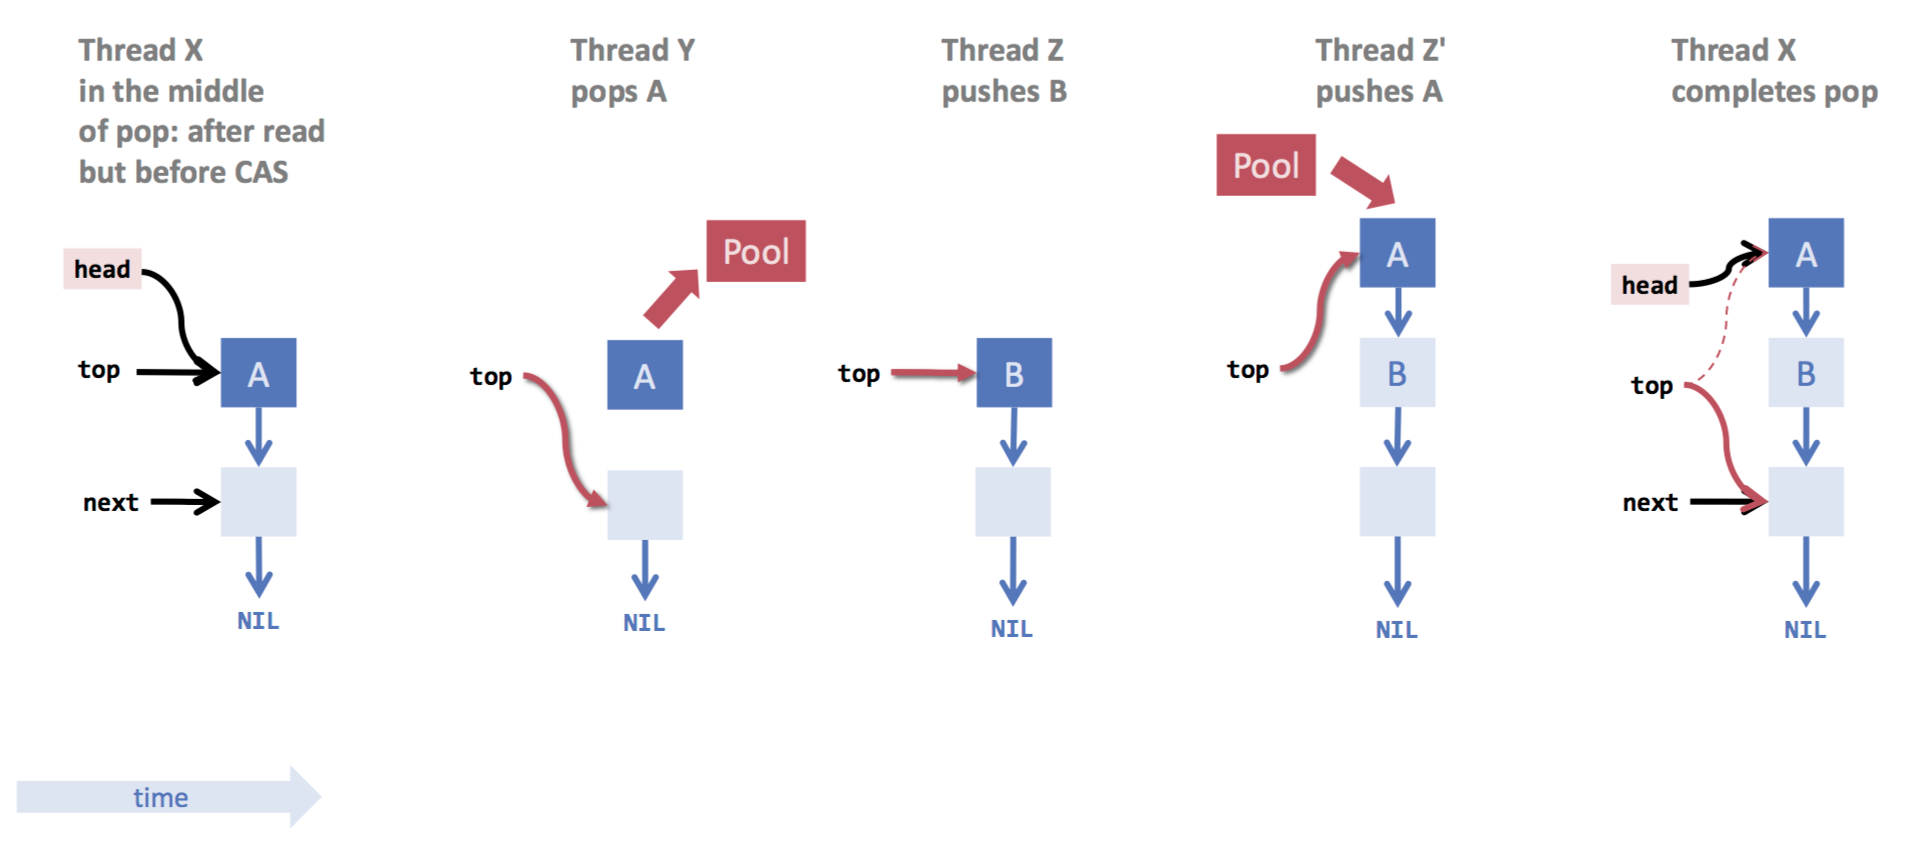
\includegraphics[width=400pt]{images/aba}
\end{center}

\begin{table}[H]
\centering
\begin{tabular}{lll}
                                 & \textbf{non-blocking} & \textbf{blocking} \\
\textbf{everyone makes progress} & wait-free             & starvation-free   \\
\textbf{someone makes progress}  & lock-free             & deadlock-free    
\end{tabular}
\end{table}

\section{Implementation}

\begin{table}[H]
\centering

\begin{tabular}{|p{2cm}|p{1cm}|p{5cm}|p{4cm}|}
\hline
                   & \textbf{Fair} & \textbf{Performance}                                                      & \textbf{Remark}                                \\ \hline
\textbf{Lock}      & no            & wasteful if held for a longer period due to contention, context switching & can be improved using an (exponential) backoff, not waitfree \\ \hline
\textbf{Read-Write Lock}      & -            & only useful if there are way more reads than writes & fairness needs to be implemented, starvation of the writes a problem \\ \hline
\textbf{Semaphore} &               &                                                                           &     \\ \hline                                           
\end{tabular}
\end{table}

\subsection{2-Thread Locks}

\subsubsection{Decker}

\begin{center}
	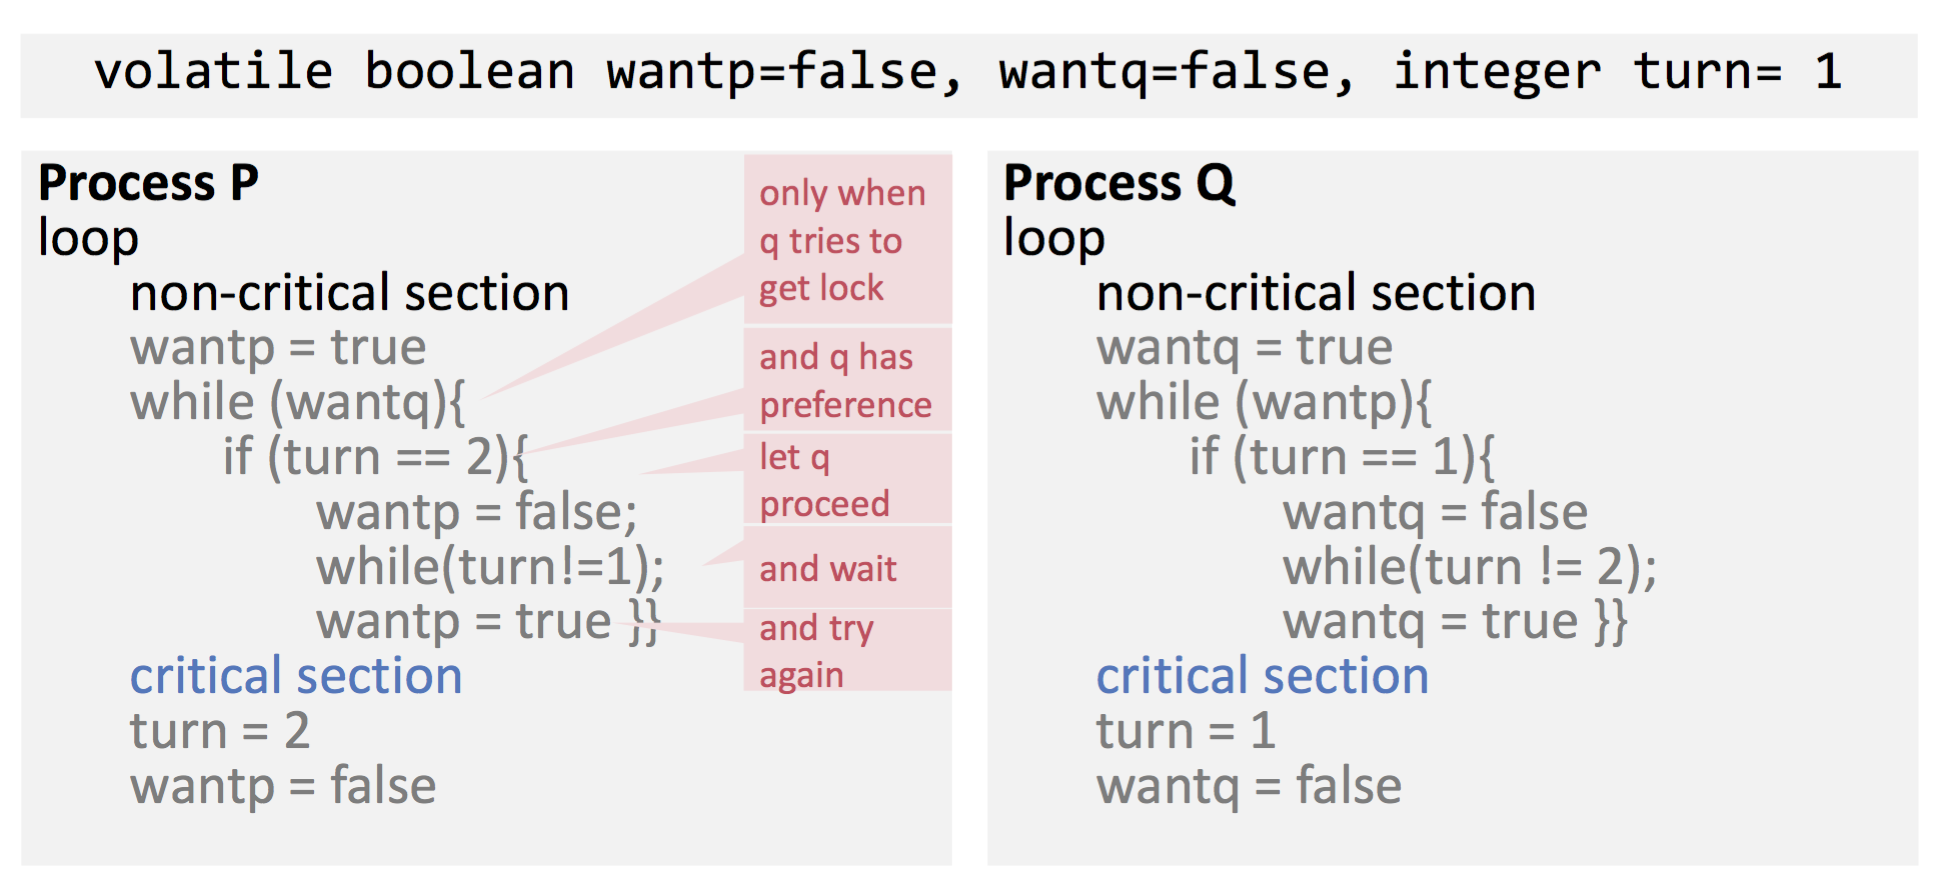
\includegraphics[width=400pt]{images/decker}
\end{center}

\subsubsection{Peterson}

\begin{center}
	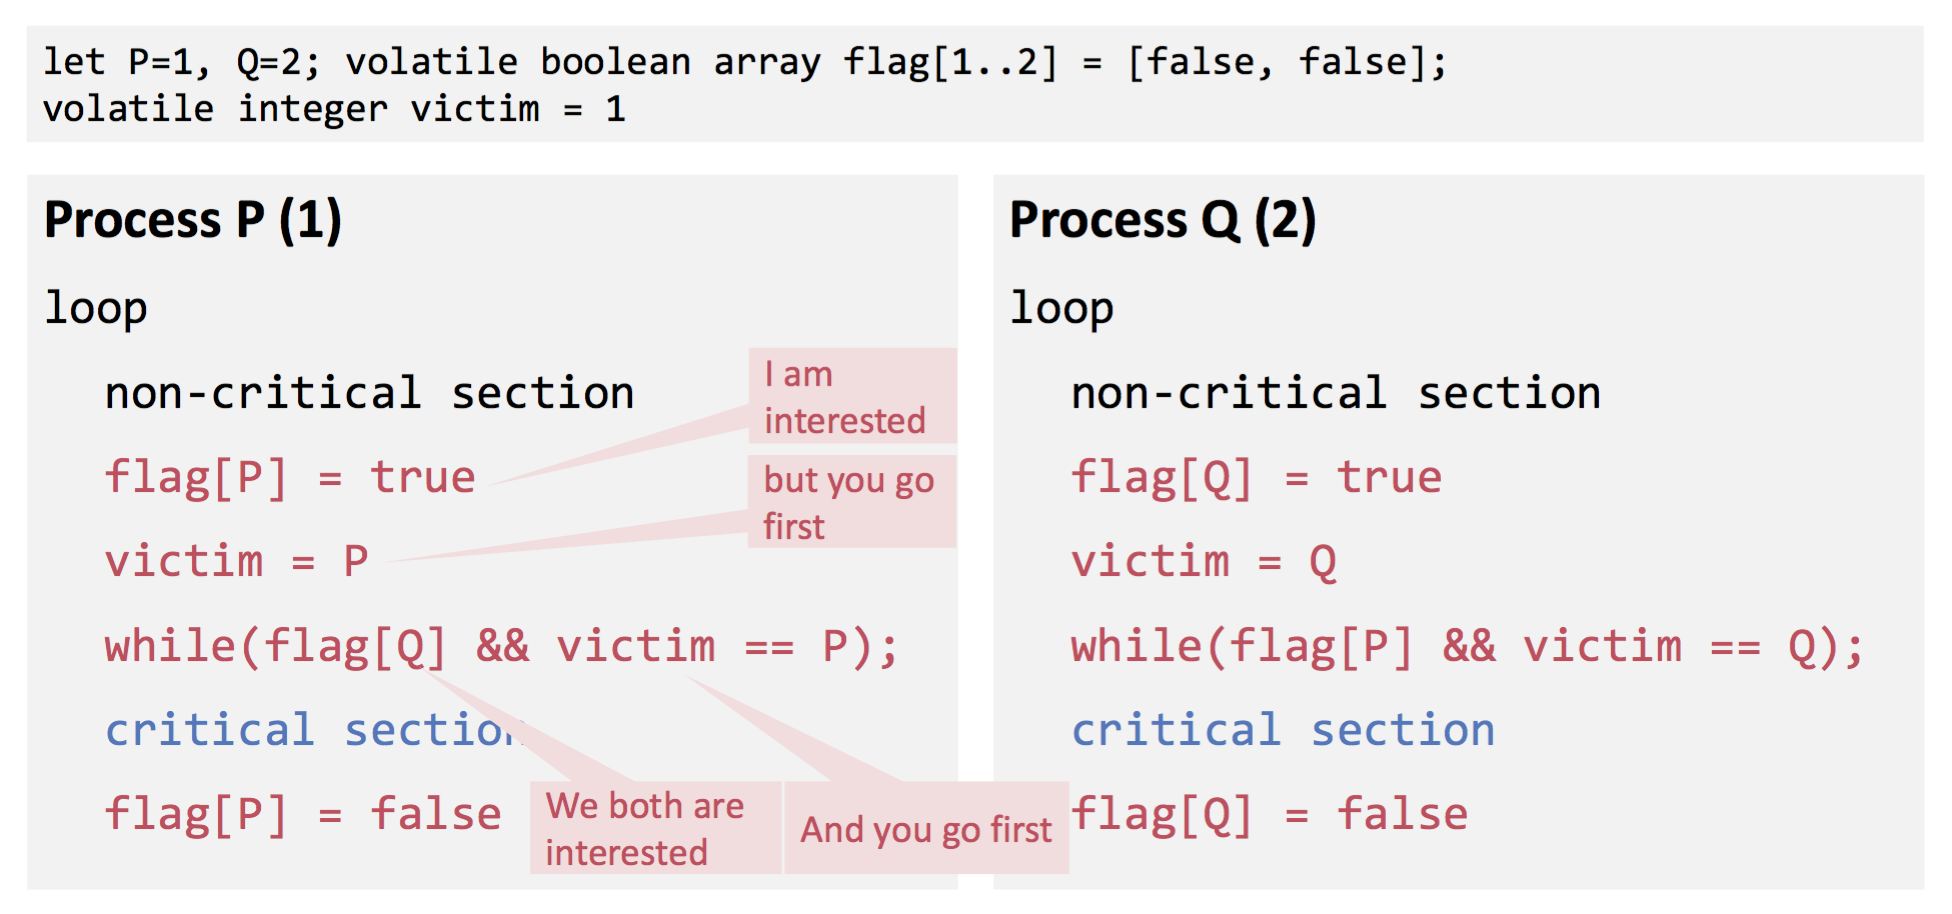
\includegraphics[width=400pt]{images/peterson}
\end{center}

\subsection{n-Thread Locks}

\subsubsection{Filter Lock}

Basically uses $n$ Peterson locks to filter $n$ threads for the critical section. It's not fair.

\subsubsection{Bakery Algorithm}

\begin{center}
	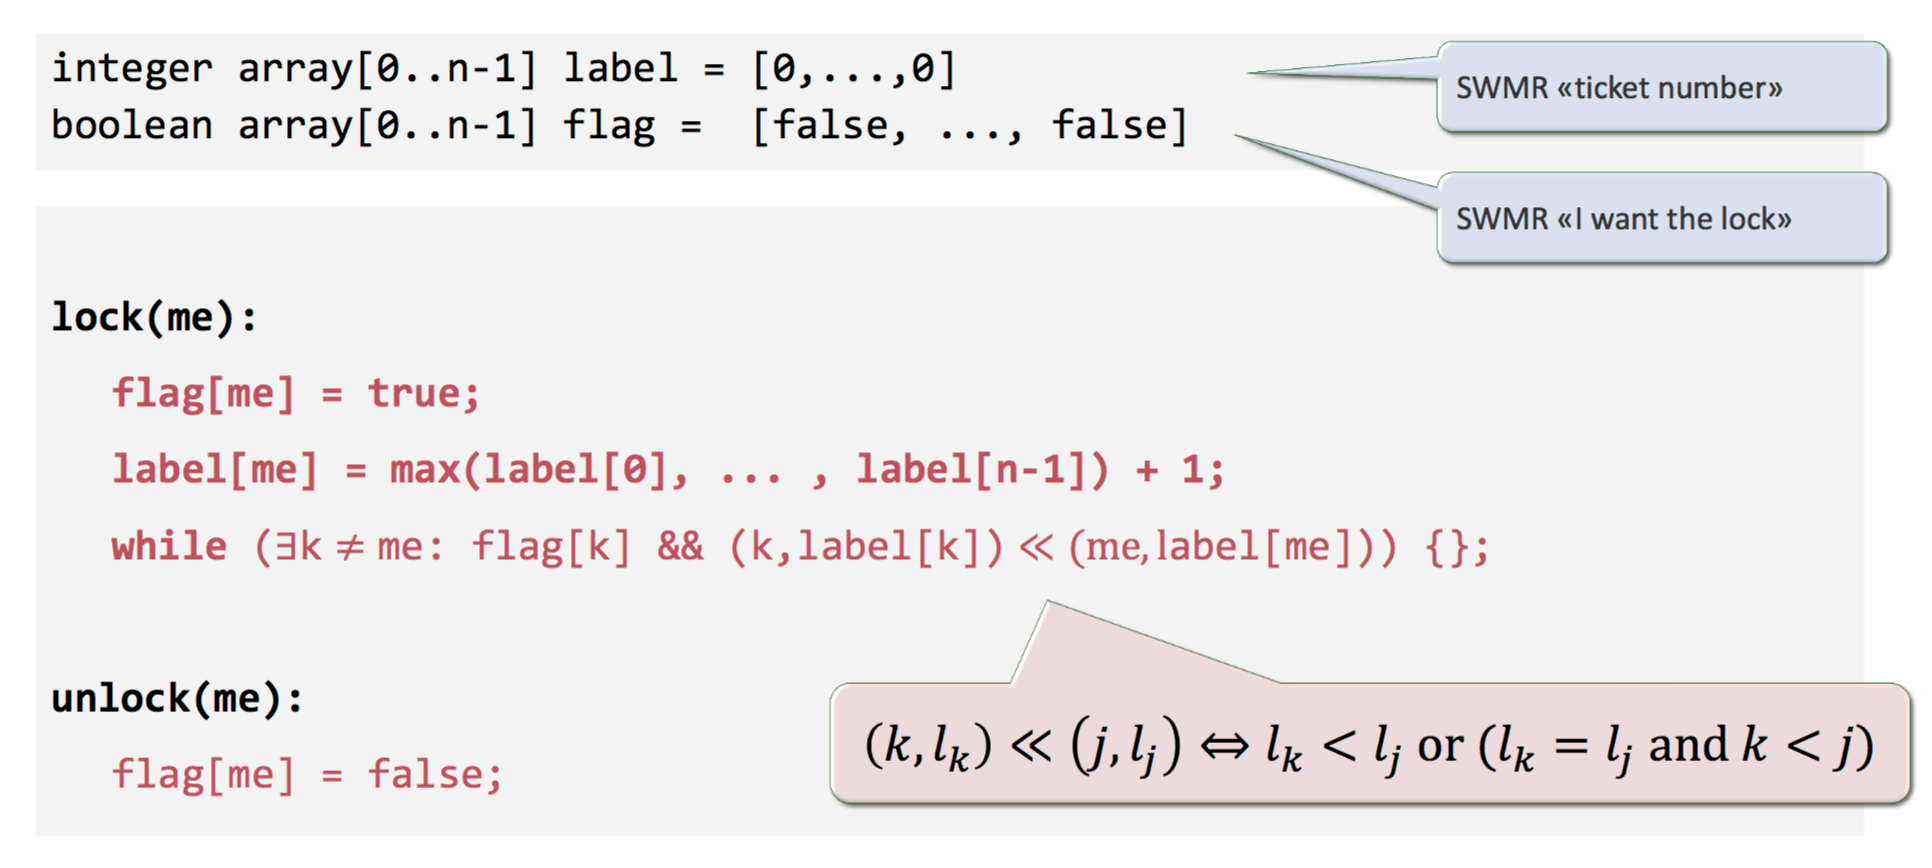
\includegraphics[width=400pt]{images/bakery}
\end{center}

\subsubsection{Spin Lock using CAS}

\begin{center}
	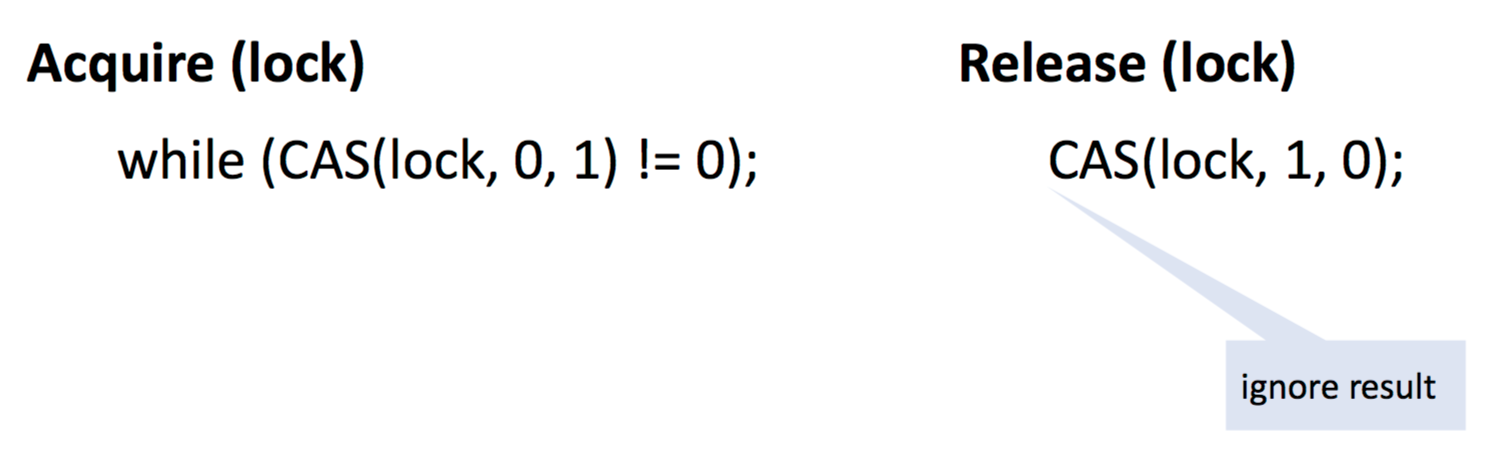
\includegraphics[width=400pt]{images/spinlock}
\end{center}

A spin lock is rather inefficient (at least if the lock is expected to be held for a longer time period). To counteract this, an \textbf{(exponential) backoff} can be implemented, so that the fighting threads don't fight over the register so much.

\section{Linearization}

\begin{description}[noitemsep]
	\item[invocation/response] method call split into two events
	\item[pending invocation] invocation that doesn't have a matching response (yet)
	\item[history H] sequence of invocations and responses
	\item[object projection H|q] history H filtered by all invocations/responses addressing q
	\item[thread projection H|B] history H filtered by all invocations/responses executed on B
	\item[complete subhistories] history H without its pending invocations
	\item[sequential history] method calls of different threads do not interleave
	\item[well formed history] per thread projections are sequential
	\item[equivalent histories] per thread projections are equal (e.g. H|A = G|A, H|B = G|B)
	\item[legal history] for every object x H|x adheres to the sequential specification of x
\end{description}

\section{Message Passing}

\begin{description}[noitemsep]
	\item[Actors] send messages in parallel which makes them more isolated (e.g. Akka for Scala, Erlang)
	\item[CSP] Communicating sequential processes, send messages sequentially, more tied together, rendezvous are possible (e.g. Go)
	\item[MPI] communication protocol for parallel processes, messages may be sent asynchronously or synchronously
\end{description}

\subsection{Consensus Protocol}

\begin{description}[noitemsep]
	\item[wait-free] returns in finite time for each thread
	\item[consistent] all threads decide on the same value
	\item[valid] the common decision is an input from one thread
\end{description}
	
\end{document}
